\begin{figure}[H]
\centering
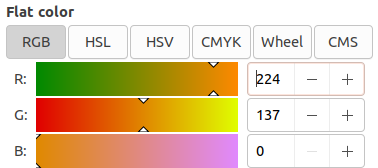
\includegraphics[width=0.6\linewidth]{figures/rgb-1}
\caption[An Example of RGB Color Values]{An example of RGB values.  If the value for red and blue are held constant, shifting the value for green up or down shifts the resulting color along the color gradient to the left of the green value, which ranges from red to yellow.  The arrows on the green gradient indicate what the current color is.  As one can see, moving the slider to the the right - increasing the value of green - will make the color more yellow, while moving it to the left, or decreasing the green level, will shift it towards orange and red.}
\label{fig:rgb-1}
\end{figure}